%W with symplectic structure
%identify W with an affine space
%more precisely, W is a vector space, A is an affine space
% lagrangian complement => equivalent to ideal


%only work with one object W, vector space, 

% make remark identifying W and K,

% do blurb, W^* \cong W 
% want to think about ring over W, 
% topology allowing algebraic geometry, allowing ring, 
% finitely many x,

% topology is allowing ring
% finite dimensional intuition
% defining an ideal in a ring

% I(LL) is an ideal of Sym(W^*)
% finite dimensions gives an isomorphism topological space

% in infinite dimensions LL point in W

%finite dimensions affine space
%infinite dimensions just have rings
%topology lets us get ring


%trying to find a point in LL, in infinite dimensions only get 0, but formal neighbourhoods can contain interesting information

%trying to solve for points, relations

%identify W and affine space

\chapter{Airy structures}
    \label{chapter:airy}
    Kontsevich and Soibelman introduce the notion of \emph{\hyperref[defn:airystruct]{Airy structures}}, \cite{ks_airy}, reproduced here in definition (\ref{defn:airystruct}), to motivate the recursive formula for topological recursion. The data from the Airy structure is then used to define \emph{\hyperref[sec:abstract_top_rec]{abstract topological recursion}}, which then for the correct choice of some initial data, specialises to give Eynard-Orantin topological recursion. 
    
    The geometric picture is that an Airy structure characterises a \emph{\hyperref[defn:quadlag]{quadratic Lagrangian}} subvariety \( \cL\) in an affine space. \( \cL \) is analogous to the zero set of a collection of quadratic polynomials. However we approach this from a more modern algebraic geometric perspective, \(\cL\) is the spectrum of a polynomial ring quotiented by an ideal generated by a collection of quadratic polynomials. However for the application to topological recursion, the \( \cL\) is represented by an ideal in a polynomial ring in infinite variables.
    
    It is possible to identify coefficients of these polynomials with tensors, denoted \(A\), \(B\), and \(C\). The fact that \( \cL\) must be Lagrangian is encoded in these tensors. Constraints on \( (A,B,C)\) is how an Airy structure is defined in \cite{ks_airy}.
    
    To get to abstract topological recursion, requires a \emph{quantum Airy structure}. Briefly, a quantum airy structure is an Airy structure, but in a non-commutative ring of operators. 
    
    In particular, the quantum Airy structures necessary for topological recursion arises from an underlying classical (in a commutative polynomial ring) Airy structure. The Poisson variety containing \( \cL\) is quantised via \emph{\hyperref[chapter:deformation]{deformation quantisation}}, as per chapter (\ref{chapter:deformation}). Naturally this gives rise to a module isomorphic to \(\mathcal{O}_\cL \) under a quotient by \( \hslash\). Along with \((A,B,C)\) from a classical Airy structure, there is an additional tensor \( \varepsilon\).
    
    Finally looking for a particular module dual to \( \mathcal{O}_{\cL} \lBrack \hslash \rBrack\) gives rise to a wavefunction, per chapter (\ref{chapter:deformation}). This wavefunction is written as \( \exp(S(x^{\sbt}))\), where \(S(x^{\sbt})\) is formal series in some parameters \(x^{\sbt}\) with coefficients built out of \( (A,B,C)\),  and \( \varepsilon\).

    \section{Lagrangian subvarieties}
    
    We consider an algebraic analog of a Lagrangian sub vector space in a symplectic vector space. First, we recall the definition of Lagrangian in the symplectic vector space setting. Let \((W,\omega)\) be a symplectic vector space. Let \(L \subset W\) be a sub vector space. Recall the \emph{symplectic complement}, \(L^{\perp}\) of \(L\) is defined as: 
    \[ L^{\perp} = \{ w \in W | \omega(w,v) = 0 , \forall v \in W\}.\]
    \begin{defn}[Coisotropic vector space]
    \label{defn:coisovect}
    \(L \) is \emph{coisotropic} if \( L^{\perp} \subset L\).
    \end{defn}
    Then \(L\) is \emph{Lagrangian}, if it is maximally coisotropic:
    \begin{defn}[Lagrangian vector space]
    \label{defn:lagrangianvect}
    \(L \) is Lagrangian if \(L = L^{\perp}\).
    \end{defn}
    Note definition (\ref{defn:lagrangianvect}), applies for arbitrary dimensional \(W\). In finite dimensions it is a consequence that \(L\) is half the dimension of \(W\).    
    
    %Let \(V\) be to a topological vector space. Let \(W \cong V \oplus V^*\) be a symplectic vector space (or Tate space), and consider the sheaf of rings over \(W\), \( \mathcal{O}_W\) as chapter \ref{chapter:tate}.
    Now consider a Poisson scheme \( (W, \mathcal{O}_W)\). For a closed subscheme \(\cL\) in \(W\) defined by an ideal sheaf \(\mathcal{J}\) of \( \mathcal{O}_W\)-modules,
    \( \mathbb{L} = \mathrm{supp}( \mathcal{O}_W/\mathcal{J})\),
    \( \mathbb{L}\) is \( \emph{coisotropic}\) if \( \mathcal{J}\) satisfies the following:
    
    %Then, the support Z of OX/J is a closed subspace of X, and (Z, OX/J) is a scheme (both assertions can be checked locally). It is called the closed subscheme of X defined by J
    
    \begin{defn}[Coisotropic subvariety] 
    \label{defn:lagrangian}
    \( \cL \) is \emph{coisotropic} in \(W\) if the ideal sheaf \(\mathcal{J}\) is closed under the Poisson bracket \[ \{ \mathcal{J} , \mathcal{J} \} \subseteq \mathcal{J}.\]
    \end{defn}
    Alternatively \( \mathcal{J}\) acting as a Poisson derivation  \( \{ \mathcal{ J} , \cdot \} \) on \( \mathcal{O}_W\) fixes \( \mathcal{J}\). Like the vector space example, Lagrangians in the algebraic picture are required to be coisotropic. To obtain what it means to be Lagrangian, we will use something which is analogous to half-dimensional. 
    
    Now suppose there are Darboux coordinates on \(W\), so \( \mathcal{O}(W) = \mathbf{k}[x_{\sbt}]  \otimes_{\mathbf{k}} \mathbf{k} [y_{\sbt}]\), and potentially an ind or pro-infinite completion along the \(x\) and \(y\) directions respectively. In the case of Airy structures, we consider Lagrangians to mean coisotropic varieties, which can locally be solved for each \(y_i\):
    \begin{defn}[quadratic Lagrangian]
    \label{defn:quadlag}
    \( \cL\) is a \emph{quadratic} Lagrangian if its defining ideal, choosing local coordinates \( (x^i,y_j)\), is generated by irreducible quadratic polynomials, \( \mathcal{J}(U) = \langle H_i : \mathcal{O}_W(U) \rangle \),  of the form 
    \[ H_i := -y_i + a_{ijk} x^j x^k + 2 b_{ij}^k x^j y_k + c_i^{jk} y_j y_k,\]
    such that \( \{ H_i , H_j \} = g_{ij}^k H_k\) for some \(g_{ij}^k \in \mathbf{k}\). Furthermore, there is a bijection between the index set of the \(H_i\) and the \(y_i\).
    \end{defn} 
    The bijection means there is an equation for each \(y_i\), and so this is analogous to half dimensional.
    
    So as long as there is a bijection between the set of \(y_{\sbt}\) coordinates, and a labelling of the defining equations for a subvariety, and as long as they satisfy the coisotropic condition, we consider this as a Lagrangian.
    %In the affine case \( \mathcal{J}\) is a prime ideal.
    
    The important property is to be able to write the Lagrangian as a local generating function \( y_i dx^i = d S_0(x^{\sbt})\), which involves solving for each \(y_i\) as a function of \(x^{\sbt}\). This means having an equation for each \(y_i\).

    This definition naturally generalises to cubic, quintic and higher order Lagrangian. 
    Instead of \( -y_i + Q_i(x^{\sbt},y_{\sbt})\) where \(Q_i\) is quadratic, it is possible to consider \( -y_i + P_i(x^{\sbt},y_{\sbt})\) for some arbitrary order polynomial \(P\). However there will be  constraints on the coefficients.
    \cite{higherairy}.
    
    An insight of Kontsevich and Soibelman is that the coeffients \(a_{ijk}, b_{ij}^k, \) and \( c_{i}^{jk}\) have  interesting structure which they term an \emph{\hyperref[defn:airystruct]{ Airy structure}}. 
    

    \section{Airy structures}




    \subsection{Affine case}
    Consider a Tate space \(W\), with possibily infinite dimensional coordinate ring (given by pro or indinfinite completions, lemma (\ref{lem:coordring})) \( \mathcal{O}(W) = \mathbf{k}[x^{\sbt},y_{\sbt}]\), where \(x^{\sbt}\), \(y_{\sbt}\) are Darboux coordinates such that there is a Poisson bracket \( \{y_i , x^j \} = \delta_i^j, \{x^i,x^j\} = \{y_i,y_j\} = 0\) . Consider the ideal \(I \) in \( \mathcal{O}(W)\), defined by the irreducible quadratic polynomials: 
    \[ I = \langle H_i = -y_i + a_{ijk} x^j x^k + 2 b_{ij}^k x^j y_k + c_i^{jk} y_j y_k \in  \mathcal{O}(W)\rangle, \] 
    with the requirement that \(I\) is closed under the Poisson bracket. Closure under the Poisson bracket is computable in terms of \(H_i\):
    \[ \{ H_i, H_j \} = g_{ij}^k H_k, \]
    where \( g_{ij}^k \) are constants. This puts constraints on the coefficients \( (a_{ijk},b_{ij}^k, c_{i}^{jk})\). 

    Further the ideal defines a \( \mathcal{O}(W) \)-module, \( \mathcal{O}(W)/I\), and  the support of this module defines a quadratic Lagrangian \( \cL \): \[ \cL  := \mathrm{supp}( \mathcal{O}(W)/I ) \cong \Spec( \mathcal{O}(W)/I ) .\]
    
    With respect to the polarisation, which is the choice of \(V\subset W\) such that \(W\cong V\oplus V^*\), the coefficients \((a_{ijk},b_{ij}^k,c_{i}^{jk})\) of \(H_i\)  can be identified with tensors:
    \begin{alignat*}{3}  
    \label{airytensor}
    A & =(a_{ijk}) && = a_{ijk}x^i \otimes x^j \otimes x^k && : \,  \Sym(V\otimes V\otimes V),\\
    B & =(b_{ij}^k) && = b_{ij}^k x^i \otimes x^j \otimes y_k &&  :\,  \Sym( V^*\otimes V\otimes V),\\   
    C & =(c_i^{jk}) && = c_i^{jk}x^i \otimes y_j \otimes y_k &&  :\,  \Sym( V^*\otimes V^*\otimes V),
    \end{alignat*}
    where repeated indicies denote summation.
    
    The closure of the Poisson bracket induces constraints on the tensors \(A\), \(B\) and \(C\). These constraints are known as an \emph{Airy structure} on \(V\) \cite{ks_airy, abcd}:  

    \begin{defn}[Airy structure]\label{defn:airystruct} An Airy structure on \(V\) is a collection of tensors \( (a_{ijk},b_{ij}^k,c_i^{jk})\) satisfying the constraints:
    \begin{align*}
       2 \left(  b_{ji}^k - b_{ij}^k \right) &= g_{ij}^k,\\
       4\left( a_{jks} b_{it}^k -  a_{iks} b_{jt}^k \right) &=  g_{ij}^k  a_{kst}, \\
       2\left(  a_{jks} c_i^{k t} -  a_{ik s} c_j^{k t} +  b_{is}^k b_{jk}^t  -  b_{ik}^t b_{js}^k \right) & =  g_{ij}^k b_{ ks}^t, \\ 
       2 \left( b_{jk}^s c_i^{kt}  - b_{ik}^s c_j^{kt}+b_{jk}^t c_i^{ks}  - b_{ik}^t c_j^{ks}\right) &= g_{ij}^k c_k^{st}.
    \end{align*}


    \end{defn}
    These constraints are homogeneous in \(A\), \(B\) and \(C\). The constraints are computed in appendix (\ref{appendix:airy}).


    %The \(H_i\)
    %define the quadratic Lagrangian subvariety \(\mathcal{L}\) in \(W\). Denote \( \mathbf{k}[\mathcal{L}]=\mathbf{k}[W]/\langle H_i \rangle \), so
    %\[ \mathrm{supp}(\mathbf{k}[\mathcal{L}] )= \mathrm{Spec} \left( \mathbf{k}[W]/\langle H_i \rangle \right)\]
    
    We are interested in studying \( \cL\) in formal neighbourhoods of the origin. Corresponding to \(\cL \) is a formal scheme \( \widehat{\cL \hspace{0pt} } \) which is given by completion of \(\cL \) by a maximal ideal \( \mathfrak{m}\) (zero in \(W\)). Concretely this is given by taking the colimit of the quotient: 
    \[ \widehat{\cL} = \colim_n  \mathrm{Spec} \left( \mathcal{O}(\cL )/\mathfrak{m}^n \right). \]
    %frac{ \mathbf{k}[ x_{\sbt} , y^{\sbt} ]}{ \langle H_i \rangle / \mathrak{m}^n } 
    The resulting formal power series describing this object contains useful information. 
    \begin{prop}The formal completion is given by
    \[ \widehat{\cL} \simeq \Spf \left(\widehat{\mathcal{O}}( W) /\langle y_i - u_{0;i}(x^{\sbt} \rangle \right), \]
    where the \(u_{0;i}\) are given by solving \(H_i= 0\) for \(y_i\) as a function of the \(x^i\), so \( y_i = u_{0,i}(x^{\sbt}) \).
    \end{prop}
        
    \begin{rem}
    This series contains the genus zero information of topological recursion.
    \end{rem}    
    %completion is flat

    
    
    \begin{rem}
    The \(n\)-th formal neighbourhood corresponds to the quotient \( \mathcal{O}(\cL)/\mathfrak{m}^n\). We think of \( \widehat{\cL} \) in terms of formal neighbourhoods.
    \end{rem}
    
    Recall, \emph{fixed point iteration} of a function \(f\) is a sequence of points \(w_n\), such that \(w_{n} = f(w_{n-1})\). If \(f\) is continuous then the fixed point \(w\) satisfies \(w=f(w)\). Completing the Hamiltonians at the maximal ideal can be viewed as a fixed point problem
    \[ y_i = f_i(y_{\sbt},x^{\sbt})\]
    where \(f_i\) are the remaining degree \(2\) terms in \(x^{\sbt}\) and \(y_{\sbt}\). 
    
    In general, the formal series \(u_{0;i}\) can be constructed via a fixed point iteration, which is equivalent to the zero genus part of Theorem 2.4.2 in \cite{ks_airy}. The point \(y^{\sbt} = 0\) is satisfied by the equation \( 0 = f_i(0,x^{\sbt})\).
    
    \begin{thm}
    The formal completion is described by the fixed point iteration:
    \begin{align*} 
    u_{0;i}^{(0)} &= a_{ijk} x^j x^k \\
    u_{0;i}^{(n)} &= a_{ijk} x^j x^k + 2 b_{ij}^k x^j u^{(n-1)}_{0;k} + c_{i}^{jk} u^{(n-1)}_{0;j} u^{(n-1)}_{0,k}.
    \end{align*}
    \end{thm}
    
    \begin{prop}
    Coefficients of this formal series stabilise: \( u^{(n)}_{0;i}(x^{\sbt}) \) converges to \( u_{0;i}(x^{\sbt}) \)
    \end{prop}
    
    Converges mean the coefficients of corresponding terms for the same degree in \(x^{\sbt}\) are equal. This is originally proven in \cite{ks_airy} more generally in terms of \emph{abstract topological recursion}. 
     
    
    
    %which can be proven inductively. \(u_0\) starts from a cubic term. 

    
    \begin{ex}
    \label{example:conic_airy}
    Consider the conic \(-y + a x^2 + 2 b x y + c y^2 = 0\) in \( \mathbf{k}[ x,y]\). 
    
    Any choice of \( (a,b,c) \) satisfies the Airy structure constraints. Solving for \(y(x)\) at \( (x,y)=(0,0)\), there is a formal solution:
    \[ u_0(x) = \frac{1}{2\, c } \left( 1 -  2\,b \,x - \sqrt{-4\, a\, c\, x^2 + (-1+2 \,b\,x)^2} \right) .\]
    \begin{itemize}
        \item If \( (a,b,c) = (1,1,1)\), this is the generating function for Catalan numbers: 
        \[ u_0(x) = x^2 + 2 x^3 + 5 x^4 + 14 x^5 + 42 x^6 + \cdots + \frac{(2n)!}{(n+1)!n!} x^{n+1}  + \cdots, \]
        as seen in chapter (\ref{chapter:deformation}).
        These numbers count rooted binary trees \cite{catalan}. 
        
        Alternatively multiplying by \(x\), this is the generating formula for the number of tri-valent graphs weighted by  \((a,b,c)\).
        
        \item If \( (a,b,c) = (1,1/2,1)\), this is the generating function for Motzkin numbers. The \(n\)-th Motzkin number counts the number of ways of drawing non-intersecting chords between \(n\) points on a circle
        \cite{motzkin}.
    \end{itemize}
    Note at \((x,y)=(0,1)\) there is another solution for the positive square root.
    \end{ex}


    The two dimensional case with scalar coefficients \((a,b,c)\), per example (\ref{example:conic_airy}) is suitable for reconstructing any example.

    %The tangent space to \( \mathcal{L} \) is given by setting \(y_i = 0\), which should recover \(L\).
    
    %More generally, \(\mathcal{L}\) is given by a localisation and a completion  \(  \lim_{\leftarrow} \mathbf{k}[W] / \mathcal{I}^n \), where \(\mathcal{I}\) is a Poisson ideal  \(\mathcal{I} = \langle H_i \rangle \). Specifically this gives a formal power series \( S_0 \in \mathbf{k} \llbracket x^{\sbt}\rrbracket\) which is zero on \(L\).
    
    % gauge transformations of airy structures

    
    Defining \( u_0(x^{\sbt}) = u_{0;i}(x^{\sbt}) x^i \), monomials can be identified with tensors in \( \widehat{\mathrm{Sym}}(V) \). The first few coefficients of \(u_0\) are 
    \[ \{ a_{ijk} , 2 b^k_{ij} a_{krs} , c_i^{jk} a_{jrs} a_{ktu}  +  4 b_{ij}^{k} b_{kr}^s a_{s tu} , \dots \}. \]
    \begin{rem}
    Note that in the infinite dimensional case, we explicitly only consider tensors such that contractions are terminating or finite sums. There is no convergence issue. In particular this is a result of the discrete topology on \(V\). Although there are infintiely many \(x^i\), a term like \(a_{ijk} x^i x^j x^k\) must only be a finite sum of different \(x^i\).
    \end{rem}
    
    \subsection{Generating function}    
    
    Generally, any Lagrangian subvariety can be represented locally by a generating function. This means take the formal completion of \( \mathcal{O}(\cL)\), at a maximal ideal corresponding to a point. In the case of the quadratic Lagrangian defined by some quadratic polynomials of \(x^{\sbt}\) and \(y^{\sbt}\), for example in one dimension (\ref{example:conic_airy}), this is analogous to solving for \(y_{\sbt}\) as a series \(u_0(x^{\sbt})\). Related to this generating function \( u_0(x^{\sbt})\) is a \emph{primitive}:
    
    \begin{defn}[Primitive] Define the \emph{primitive} \( S_0(x^{\sbt})\) as the function such that \( d S_0(x^{\sbt}) = u_{0,i}(x^{\sbt}) dx^i\).
    \end{defn}
    
    This primitive is related to the symplectic form.
    
    The restriction of a primitive of a symplectic form to a Lagrangian subvariety is exact. In the case of a symplectic variety, there is a symplectic form \( \Omega = d ( - y_i  dx^i)= - d y_i \wedge d x^i \).
    
    Restrict the primitive, \(-y_idx^i\), of \(\Omega\), to a formal neighbourhood of \(0\in \widehat{\cL}\) to get a function \(S_0\) defined in a neighbourhood in \(W\) of \(0 \in \widehat{\cL}\) satisfying:
    \[y_idx^i:=dS_0(x^{\sbt}) = u_{0;i}(x^{\sbt}) dx^i.\]
    Explicitly writing out some terms gives:
    \[S_0(x)=\frac{1}{3} a_{ijk}x^ix^jx^k+\frac{1}{6} \left(b_{ij}^k a_{k\ell m}+b_{i\ell}^k a_{kj m}+b_{im}^ka_{kj\ell}\right)x^ix^jx^\ell x^m + \dots.
    \]
    \begin{lem}
        \(S_0(x^{\sbt})\) is symmetric under permutations of the \( x^{\sbt}\), which in finite and infinite dimensions, corresponds to bijections of the index set \( I \rightarrow I\).
    \end{lem}
    The symmetry of \(S_0(x^{\sbt})\) is a consequence of \( \{ H_i, H_j \} = g_{ij}^k H_k\).  Differentiating \(S_0\) with respect to \(x_i\) generates other identities involving the tensors
    \[ (a_{ijk},b_{ij}^{k}, c_{i}^{jk}),\]
    which also follow from the closure condition. 
    For example:
    \[ b_{ij}^ka_{k\ell m}+b_{i\ell}^ka_{kj m}+b_{im}^ka_{kj\ell}= b_{ji}^ka_{k\ell m}+b_{j\ell}^ka_{ki m}+b_{jm}^ka_{ki\ell},
    \]
    which agrees with the constraints in definition (\ref{defn:airystruct}). For example we see that
    \[\frac{\partial}{\partial x^i} S_{0,4}=\frac{4}{6}(b_{ij}^ka_{k\ell m}+b_{i\ell}^ka_{kj m}+b_{im}^ka_{kj\ell})x^jx^\ell x^m= 2 b_{ij}^ka_{k\ell m}x^jx^\ell x^m=u_{0,i}^{(4)}\]
    as required.  
    
    
    % F_0 prepotential
    
    
    \subsection{Graphical representation}
    
    There is a diagrammatic, or graphical, algorithm to compute the monomials \( u_{0,n; i}(x^{\sbt})\). Previously, topological recursion has been visualised as a graphical sum, for example \cite{eynard_orantin}, so we outline a similar scheme for the function \(u_0(x)\) encoding the Lagrangian in the case of Airy structures. 

    In the case of the planar conic, 
    \[ -y + x^2 + 2 \,x \,y + y^2 \in  \mathbf{k}[x,y],\]
    solving for \(y(x)=0\) as a power series in \(x\), gives the generating function for Catalan numbers, which count rooted binary trees. Associated to these numbers, in chapter (\ref{chapter:deformation}), we drew the trees up to isomorphism. A weighted count of these trees, returns the Catalan numbers, which are the coefficients of powers of \(x\) in \(y(x)\).  The same process can be carried out with the weighted conic 
    \[ - y + a \, x^2  + 2 \, x\,y + c \, y^2,\]
    which assigns a particular weighting of certain trees. This conic is nearly sufficient for even producing the coefficients of the \(2n\) or even infinite dimensional case of solving for \(y_{\sbt}\) in the quadratics \(H_{\sbt}\) in \( \mathbf{k}[x^1, \dots , y_1, \dots ]\). To recover the tensor contractions in the coefficients of products of \(x^{\sbt}\), requires something like \emph{type-inference}.  The weighted conic gives the correct structure but forgets information about the tensor contractions.
    
    In this section we describe a procedure to find the coefficients in \( u_{0,n,i}\). Coefficients of \(x^{\sbt}\) in \(u_{0,i}\) are identifiable with rooted trees, much like the \(1\) dimensional case 
    \(  - y + a \, x^2  + 2 \, x\,y + c \, y^2\), but we have to infer the tensor contractions. 
    
    To do this, we will consider building a directed graphs from the trees, and then use this to assign a certain labelling to vertices. 
    
    Generating trees up to isomorphism type, and counting types weighted by number of automorphisms will generate Catalan numbers.
    %So \( u_{0,n;i} \) is a similar collection of rooted trees, but we will consider these as directed graphs, with one special vertex, and with zero genus. 
    Furthermore, the purpose of considering graphs instead of trees is to examine a generalisation required in the case of quantum Airy structures.
    
    \subsubsection{Generating graphs}
    
    To build the graphs corresponding to \( u_{0,n; i}\), for \( n \geq 3\), we start with undirected graphs in \(2n-2\) vertices, comprising of \(n\) degree \(1\) vertices, and \(n-2\) degree \(3\) vertices. Note that we only consider graphs up to automorphism.
    
    From the undirected graphs, generate a collection of graphs where an orientation is chosen on every edge. The orientation of an edge in the graph is denoted with an arrow. Relative to a vertex, we call an edge incoming if the arrow points in towards the vertex \( (\rightarrow \sbt) \), or outgoing if pointing away \( ( \leftarrow \sbt)\). Incoming edges we label with orientation \(-1\), outgoing with \(+1\).  
    
    Every degree \(1\) vertex in the original undirected graph must be given an incoming edge, for example figure (\ref{fig:apply_orient}). 
    \begin{figure}[h!]
        \centering
        

\tikzset{every picture/.style={line width=0.75pt}} %set default line width to 0.75pt        

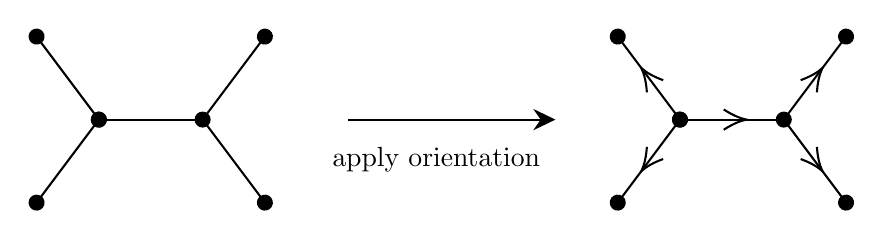
\begin{tikzpicture}[x=0.75pt,y=0.75pt,yscale=-1,xscale=1]
%uncomment if require: \path (0,111); %set diagram left start at 0, and has height of 111

%Straight Lines [id:da741919041298036] 
\draw    (40,50) -- (10,90) ;
\draw [shift={(10,90)}, rotate = 126.87] [color={rgb, 255:red, 0; green, 0; blue, 0 }  ][fill={rgb, 255:red, 0; green, 0; blue, 0 }  ][line width=0.75]      (0, 0) circle [x radius= 3.35, y radius= 3.35]   ;
\draw [shift={(40,50)}, rotate = 126.87] [color={rgb, 255:red, 0; green, 0; blue, 0 }  ][fill={rgb, 255:red, 0; green, 0; blue, 0 }  ][line width=0.75]      (0, 0) circle [x radius= 3.35, y radius= 3.35]   ;
%Straight Lines [id:da47409531598256205] 
\draw    (40,50) -- (10,10) ;
\draw [shift={(10,10)}, rotate = 233.13] [color={rgb, 255:red, 0; green, 0; blue, 0 }  ][fill={rgb, 255:red, 0; green, 0; blue, 0 }  ][line width=0.75]      (0, 0) circle [x radius= 3.35, y radius= 3.35]   ;
%Straight Lines [id:da2399175289181944] 
\draw    (90,50) -- (120,90) ;
\draw [shift={(120,90)}, rotate = 53.13] [color={rgb, 255:red, 0; green, 0; blue, 0 }  ][fill={rgb, 255:red, 0; green, 0; blue, 0 }  ][line width=0.75]      (0, 0) circle [x radius= 3.35, y radius= 3.35]   ;
%Straight Lines [id:da483679229546244] 
\draw    (90,50) -- (40,50) ;
\draw [shift={(40,50)}, rotate = 180] [color={rgb, 255:red, 0; green, 0; blue, 0 }  ][fill={rgb, 255:red, 0; green, 0; blue, 0 }  ][line width=0.75]      (0, 0) circle [x radius= 3.35, y radius= 3.35]   ;
\draw [shift={(90,50)}, rotate = 180] [color={rgb, 255:red, 0; green, 0; blue, 0 }  ][fill={rgb, 255:red, 0; green, 0; blue, 0 }  ][line width=0.75]      (0, 0) circle [x radius= 3.35, y radius= 3.35]   ;
%Straight Lines [id:da6663059195826004] 
\draw    (120,10) -- (90,50) ;
\draw [shift={(120,10)}, rotate = 126.87] [color={rgb, 255:red, 0; green, 0; blue, 0 }  ][fill={rgb, 255:red, 0; green, 0; blue, 0 }  ][line width=0.75]      (0, 0) circle [x radius= 3.35, y radius= 3.35]   ;
%Straight Lines [id:da7084400491516926] 
\draw    (320,50) -- (290,90) ;
\draw [shift={(290,90)}, rotate = 126.87] [color={rgb, 255:red, 0; green, 0; blue, 0 }  ][fill={rgb, 255:red, 0; green, 0; blue, 0 }  ][line width=0.75]      (0, 0) circle [x radius= 3.35, y radius= 3.35]   ;
\draw [shift={(301.4,74.8)}, rotate = 306.87] [color={rgb, 255:red, 0; green, 0; blue, 0 }  ][line width=0.75]    (10.93,-4.9) .. controls (6.95,-2.3) and (3.31,-0.67) .. (0,0) .. controls (3.31,0.67) and (6.95,2.3) .. (10.93,4.9)   ;
\draw [shift={(320,50)}, rotate = 126.87] [color={rgb, 255:red, 0; green, 0; blue, 0 }  ][fill={rgb, 255:red, 0; green, 0; blue, 0 }  ][line width=0.75]      (0, 0) circle [x radius= 3.35, y radius= 3.35]   ;
%Straight Lines [id:da21676438064922232] 
\draw    (320,50) -- (290,10) ;
\draw [shift={(290,10)}, rotate = 233.13] [color={rgb, 255:red, 0; green, 0; blue, 0 }  ][fill={rgb, 255:red, 0; green, 0; blue, 0 }  ][line width=0.75]      (0, 0) circle [x radius= 3.35, y radius= 3.35]   ;
\draw [shift={(301.4,25.2)}, rotate = 53.13] [color={rgb, 255:red, 0; green, 0; blue, 0 }  ][line width=0.75]    (10.93,-4.9) .. controls (6.95,-2.3) and (3.31,-0.67) .. (0,0) .. controls (3.31,0.67) and (6.95,2.3) .. (10.93,4.9)   ;
%Straight Lines [id:da40569083986374777] 
\draw    (370,50) -- (400,90) ;
\draw [shift={(400,90)}, rotate = 53.13] [color={rgb, 255:red, 0; green, 0; blue, 0 }  ][fill={rgb, 255:red, 0; green, 0; blue, 0 }  ][line width=0.75]      (0, 0) circle [x radius= 3.35, y radius= 3.35]   ;
\draw [shift={(388.6,74.8)}, rotate = 233.13] [color={rgb, 255:red, 0; green, 0; blue, 0 }  ][line width=0.75]    (10.93,-4.9) .. controls (6.95,-2.3) and (3.31,-0.67) .. (0,0) .. controls (3.31,0.67) and (6.95,2.3) .. (10.93,4.9)   ;
%Straight Lines [id:da7723467199596994] 
\draw    (370,50) -- (320,50) ;
\draw [shift={(320,50)}, rotate = 180] [color={rgb, 255:red, 0; green, 0; blue, 0 }  ][fill={rgb, 255:red, 0; green, 0; blue, 0 }  ][line width=0.75]      (0, 0) circle [x radius= 3.35, y radius= 3.35]   ;
\draw [shift={(352,50)}, rotate = 180] [color={rgb, 255:red, 0; green, 0; blue, 0 }  ][line width=0.75]    (10.93,-4.9) .. controls (6.95,-2.3) and (3.31,-0.67) .. (0,0) .. controls (3.31,0.67) and (6.95,2.3) .. (10.93,4.9)   ;
\draw [shift={(370,50)}, rotate = 180] [color={rgb, 255:red, 0; green, 0; blue, 0 }  ][fill={rgb, 255:red, 0; green, 0; blue, 0 }  ][line width=0.75]      (0, 0) circle [x radius= 3.35, y radius= 3.35]   ;
%Straight Lines [id:da9015362240911622] 
\draw    (370,50) -- (400,10) ;
\draw [shift={(400,10)}, rotate = 306.87] [color={rgb, 255:red, 0; green, 0; blue, 0 }  ][fill={rgb, 255:red, 0; green, 0; blue, 0 }  ][line width=0.75]      (0, 0) circle [x radius= 3.35, y radius= 3.35]   ;
\draw [shift={(388.6,25.2)}, rotate = 126.87] [color={rgb, 255:red, 0; green, 0; blue, 0 }  ][line width=0.75]    (10.93,-4.9) .. controls (6.95,-2.3) and (3.31,-0.67) .. (0,0) .. controls (3.31,0.67) and (6.95,2.3) .. (10.93,4.9)   ;
%Straight Lines [id:da28552551016148775] 
\draw    (160,50) -- (257,50) ;
\draw [shift={(260,50)}, rotate = 180] [fill={rgb, 255:red, 0; green, 0; blue, 0 }  ][line width=0.08]  [draw opacity=0] (10.72,-5.15) -- (0,0) -- (10.72,5.15) -- (7.12,0) -- cycle    ;

% Text Node
\draw (151,62) node [anchor=north west][inner sep=0.75pt]   [align=left] {apply orientation};


\end{tikzpicture}


        \caption{Applying the orientation in the case of \(n=4\). There is only one possible graph.}
        \label{fig:apply_orient}
    \end{figure}
    Next we consider possible orientations for the edges of the degree \(3\) vertices. Starting at a vertex with two outgoing edges, which are attached to two degree \(1\) vertices, edges are chosen for the degree \(3\) vertices in an ordered way, edges must be oriented so they form consecutive strings of \(+1\) or \(-1\), for example, for the graph in figure (\ref{fig:apply_internal}), relative to the starting vertex, the orientations:
    \[ \{ +1, +1 , +1\} ,\; \{ +1, +1 ,-1  \}, \; \{+1,-1,-1\}, \]
    are allowed, while 
    \[ \{ +1,-1,+1\},\]
    is not. This effectively generates a unique internal vertex in the graph, that all internal edges can be traversed to unambiguously. For more complicated graphs this means creating a vertex that acts as a sink. A sink is a vertex that all (internal) paths, following the orientation of the edges, lead to for example (\ref{fig:apply_internal}).
    \begin{figure}[htb]
        \centering
        

\tikzset{every picture/.style={line width=0.75pt}} %set default line width to 0.75pt        

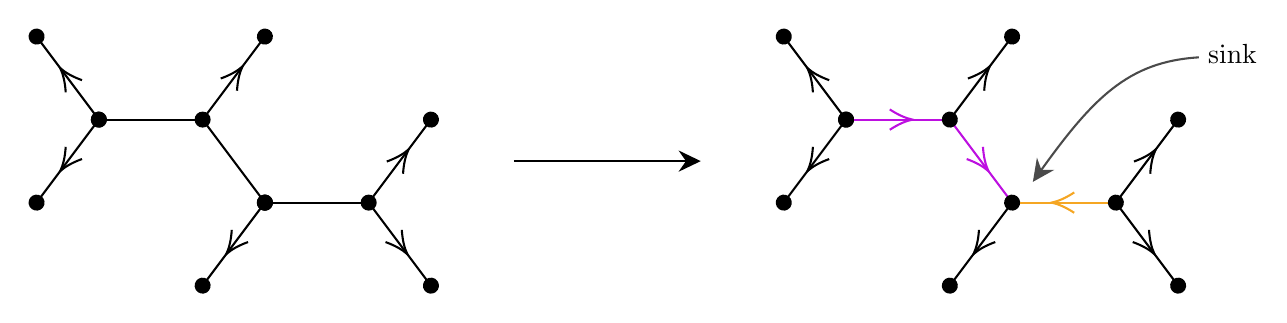
\begin{tikzpicture}[x=0.75pt,y=0.75pt,yscale=-1,xscale=1]
%uncomment if require: \path (0,151); %set diagram left start at 0, and has height of 151

%Straight Lines [id:da22627610725586034] 
\draw [color={rgb, 255:red, 189; green, 16; blue, 224 }  ,draw opacity=1 ]   (450,50) -- (400,50) ;
\draw [shift={(432,50)}, rotate = 180] [color={rgb, 255:red, 189; green, 16; blue, 224 }  ,draw opacity=1 ][line width=0.75]    (10.93,-4.9) .. controls (6.95,-2.3) and (3.31,-0.67) .. (0,0) .. controls (3.31,0.67) and (6.95,2.3) .. (10.93,4.9)   ;
%Straight Lines [id:da041653782173061815] 
\draw    (40,50) -- (10,90) ;
\draw [shift={(10,90)}, rotate = 126.87] [color={rgb, 255:red, 0; green, 0; blue, 0 }  ][fill={rgb, 255:red, 0; green, 0; blue, 0 }  ][line width=0.75]      (0, 0) circle [x radius= 3.35, y radius= 3.35]   ;
\draw [shift={(21.4,74.8)}, rotate = 306.87] [color={rgb, 255:red, 0; green, 0; blue, 0 }  ][line width=0.75]    (10.93,-4.9) .. controls (6.95,-2.3) and (3.31,-0.67) .. (0,0) .. controls (3.31,0.67) and (6.95,2.3) .. (10.93,4.9)   ;
\draw [shift={(40,50)}, rotate = 126.87] [color={rgb, 255:red, 0; green, 0; blue, 0 }  ][fill={rgb, 255:red, 0; green, 0; blue, 0 }  ][line width=0.75]      (0, 0) circle [x radius= 3.35, y radius= 3.35]   ;
%Straight Lines [id:da07326718492135587] 
\draw    (40,50) -- (10,10) ;
\draw [shift={(10,10)}, rotate = 233.13] [color={rgb, 255:red, 0; green, 0; blue, 0 }  ][fill={rgb, 255:red, 0; green, 0; blue, 0 }  ][line width=0.75]      (0, 0) circle [x radius= 3.35, y radius= 3.35]   ;
\draw [shift={(21.4,25.2)}, rotate = 53.13] [color={rgb, 255:red, 0; green, 0; blue, 0 }  ][line width=0.75]    (10.93,-4.9) .. controls (6.95,-2.3) and (3.31,-0.67) .. (0,0) .. controls (3.31,0.67) and (6.95,2.3) .. (10.93,4.9)   ;
%Straight Lines [id:da7839214017358417] 
\draw    (90,50) -- (120,90) ;
\draw [shift={(120,90)}, rotate = 53.13] [color={rgb, 255:red, 0; green, 0; blue, 0 }  ][fill={rgb, 255:red, 0; green, 0; blue, 0 }  ][line width=0.75]      (0, 0) circle [x radius= 3.35, y radius= 3.35]   ;
%Straight Lines [id:da14376202126053506] 
\draw    (90,50) -- (40,50) ;
\draw [shift={(40,50)}, rotate = 180] [color={rgb, 255:red, 0; green, 0; blue, 0 }  ][fill={rgb, 255:red, 0; green, 0; blue, 0 }  ][line width=0.75]      (0, 0) circle [x radius= 3.35, y radius= 3.35]   ;
\draw [shift={(90,50)}, rotate = 180] [color={rgb, 255:red, 0; green, 0; blue, 0 }  ][fill={rgb, 255:red, 0; green, 0; blue, 0 }  ][line width=0.75]      (0, 0) circle [x radius= 3.35, y radius= 3.35]   ;
%Straight Lines [id:da7008688072010646] 
\draw    (120,10) -- (90,50) ;
\draw [shift={(109.2,24.4)}, rotate = 126.87] [color={rgb, 255:red, 0; green, 0; blue, 0 }  ][line width=0.75]    (10.93,-4.9) .. controls (6.95,-2.3) and (3.31,-0.67) .. (0,0) .. controls (3.31,0.67) and (6.95,2.3) .. (10.93,4.9)   ;
\draw [shift={(120,10)}, rotate = 126.87] [color={rgb, 255:red, 0; green, 0; blue, 0 }  ][fill={rgb, 255:red, 0; green, 0; blue, 0 }  ][line width=0.75]      (0, 0) circle [x radius= 3.35, y radius= 3.35]   ;
%Straight Lines [id:da359668980650211] 
\draw    (170,90) -- (120,90) ;
\draw [shift={(120,90)}, rotate = 180] [color={rgb, 255:red, 0; green, 0; blue, 0 }  ][fill={rgb, 255:red, 0; green, 0; blue, 0 }  ][line width=0.75]      (0, 0) circle [x radius= 3.35, y radius= 3.35]   ;
\draw [shift={(170,90)}, rotate = 180] [color={rgb, 255:red, 0; green, 0; blue, 0 }  ][fill={rgb, 255:red, 0; green, 0; blue, 0 }  ][line width=0.75]      (0, 0) circle [x radius= 3.35, y radius= 3.35]   ;
%Straight Lines [id:da5577770273154145] 
\draw    (120,90) -- (90,130) ;
\draw [shift={(90,130)}, rotate = 126.87] [color={rgb, 255:red, 0; green, 0; blue, 0 }  ][fill={rgb, 255:red, 0; green, 0; blue, 0 }  ][line width=0.75]      (0, 0) circle [x radius= 3.35, y radius= 3.35]   ;
\draw [shift={(101.4,114.8)}, rotate = 306.87] [color={rgb, 255:red, 0; green, 0; blue, 0 }  ][line width=0.75]    (10.93,-4.9) .. controls (6.95,-2.3) and (3.31,-0.67) .. (0,0) .. controls (3.31,0.67) and (6.95,2.3) .. (10.93,4.9)   ;
\draw [shift={(120,90)}, rotate = 126.87] [color={rgb, 255:red, 0; green, 0; blue, 0 }  ][fill={rgb, 255:red, 0; green, 0; blue, 0 }  ][line width=0.75]      (0, 0) circle [x radius= 3.35, y radius= 3.35]   ;
%Straight Lines [id:da21435000458697373] 
\draw    (200,50) -- (170,90) ;
\draw [shift={(189.2,64.4)}, rotate = 126.87] [color={rgb, 255:red, 0; green, 0; blue, 0 }  ][line width=0.75]    (10.93,-4.9) .. controls (6.95,-2.3) and (3.31,-0.67) .. (0,0) .. controls (3.31,0.67) and (6.95,2.3) .. (10.93,4.9)   ;
\draw [shift={(200,50)}, rotate = 126.87] [color={rgb, 255:red, 0; green, 0; blue, 0 }  ][fill={rgb, 255:red, 0; green, 0; blue, 0 }  ][line width=0.75]      (0, 0) circle [x radius= 3.35, y radius= 3.35]   ;
%Straight Lines [id:da6194639262307314] 
\draw    (170,90) -- (200,130) ;
\draw [shift={(200,130)}, rotate = 53.13] [color={rgb, 255:red, 0; green, 0; blue, 0 }  ][fill={rgb, 255:red, 0; green, 0; blue, 0 }  ][line width=0.75]      (0, 0) circle [x radius= 3.35, y radius= 3.35]   ;
\draw [shift={(188.6,114.8)}, rotate = 233.13] [color={rgb, 255:red, 0; green, 0; blue, 0 }  ][line width=0.75]    (10.93,-4.9) .. controls (6.95,-2.3) and (3.31,-0.67) .. (0,0) .. controls (3.31,0.67) and (6.95,2.3) .. (10.93,4.9)   ;
%Straight Lines [id:da9011665660368904] 
\draw    (240,70) -- (327,70) ;
\draw [shift={(330,70)}, rotate = 180] [fill={rgb, 255:red, 0; green, 0; blue, 0 }  ][line width=0.08]  [draw opacity=0] (10.72,-5.15) -- (0,0) -- (10.72,5.15) -- (7.12,0) -- cycle    ;
%Straight Lines [id:da6450639046565149] 
\draw    (400,50) -- (370,90) ;
\draw [shift={(370,90)}, rotate = 126.87] [color={rgb, 255:red, 0; green, 0; blue, 0 }  ][fill={rgb, 255:red, 0; green, 0; blue, 0 }  ][line width=0.75]      (0, 0) circle [x radius= 3.35, y radius= 3.35]   ;
\draw [shift={(381.4,74.8)}, rotate = 306.87] [color={rgb, 255:red, 0; green, 0; blue, 0 }  ][line width=0.75]    (10.93,-4.9) .. controls (6.95,-2.3) and (3.31,-0.67) .. (0,0) .. controls (3.31,0.67) and (6.95,2.3) .. (10.93,4.9)   ;
\draw [shift={(400,50)}, rotate = 126.87] [color={rgb, 255:red, 0; green, 0; blue, 0 }  ][fill={rgb, 255:red, 0; green, 0; blue, 0 }  ][line width=0.75]      (0, 0) circle [x radius= 3.35, y radius= 3.35]   ;
%Straight Lines [id:da8590739970406319] 
\draw    (400,50) -- (370,10) ;
\draw [shift={(370,10)}, rotate = 233.13] [color={rgb, 255:red, 0; green, 0; blue, 0 }  ][fill={rgb, 255:red, 0; green, 0; blue, 0 }  ][line width=0.75]      (0, 0) circle [x radius= 3.35, y radius= 3.35]   ;
\draw [shift={(381.4,25.2)}, rotate = 53.13] [color={rgb, 255:red, 0; green, 0; blue, 0 }  ][line width=0.75]    (10.93,-4.9) .. controls (6.95,-2.3) and (3.31,-0.67) .. (0,0) .. controls (3.31,0.67) and (6.95,2.3) .. (10.93,4.9)   ;
\draw [shift={(400,50)}, rotate = 233.13] [color={rgb, 255:red, 0; green, 0; blue, 0 }  ][fill={rgb, 255:red, 0; green, 0; blue, 0 }  ][line width=0.75]      (0, 0) circle [x radius= 3.35, y radius= 3.35]   ;
%Straight Lines [id:da07942613501626583] 
\draw [color={rgb, 255:red, 189; green, 16; blue, 224 }  ,draw opacity=1 ]   (450,50) -- (480,90) ;
\draw [shift={(468.6,74.8)}, rotate = 233.13] [color={rgb, 255:red, 189; green, 16; blue, 224 }  ,draw opacity=1 ][line width=0.75]    (10.93,-4.9) .. controls (6.95,-2.3) and (3.31,-0.67) .. (0,0) .. controls (3.31,0.67) and (6.95,2.3) .. (10.93,4.9)   ;
%Straight Lines [id:da3697972639758368] 
\draw    (480,10) -- (450,50) ;
\draw [shift={(450,50)}, rotate = 126.87] [color={rgb, 255:red, 0; green, 0; blue, 0 }  ][fill={rgb, 255:red, 0; green, 0; blue, 0 }  ][line width=0.75]      (0, 0) circle [x radius= 3.35, y radius= 3.35]   ;
\draw [shift={(469.2,24.4)}, rotate = 126.87] [color={rgb, 255:red, 0; green, 0; blue, 0 }  ][line width=0.75]    (10.93,-4.9) .. controls (6.95,-2.3) and (3.31,-0.67) .. (0,0) .. controls (3.31,0.67) and (6.95,2.3) .. (10.93,4.9)   ;
\draw [shift={(480,10)}, rotate = 126.87] [color={rgb, 255:red, 0; green, 0; blue, 0 }  ][fill={rgb, 255:red, 0; green, 0; blue, 0 }  ][line width=0.75]      (0, 0) circle [x radius= 3.35, y radius= 3.35]   ;
%Straight Lines [id:da8337199770042564] 
\draw [color={rgb, 255:red, 245; green, 166; blue, 35 }  ,draw opacity=1 ][fill={rgb, 255:red, 245; green, 166; blue, 35 }  ,fill opacity=1 ]   (530,90) -- (480,90) ;
\draw [shift={(499,90)}, rotate = 360] [color={rgb, 255:red, 245; green, 166; blue, 35 }  ,draw opacity=1 ][line width=0.75]    (10.93,-4.9) .. controls (6.95,-2.3) and (3.31,-0.67) .. (0,0) .. controls (3.31,0.67) and (6.95,2.3) .. (10.93,4.9)   ;
%Straight Lines [id:da7264994944566067] 
\draw [fill={rgb, 255:red, 245; green, 166; blue, 35 }  ,fill opacity=1 ]   (480,90) -- (450,130) ;
\draw [shift={(450,130)}, rotate = 126.87] [color={rgb, 255:red, 0; green, 0; blue, 0 }  ][fill={rgb, 255:red, 0; green, 0; blue, 0 }  ][line width=0.75]      (0, 0) circle [x radius= 3.35, y radius= 3.35]   ;
\draw [shift={(461.4,114.8)}, rotate = 306.87] [color={rgb, 255:red, 0; green, 0; blue, 0 }  ][line width=0.75]    (10.93,-4.9) .. controls (6.95,-2.3) and (3.31,-0.67) .. (0,0) .. controls (3.31,0.67) and (6.95,2.3) .. (10.93,4.9)   ;
\draw [shift={(480,90)}, rotate = 126.87] [color={rgb, 255:red, 0; green, 0; blue, 0 }  ][fill={rgb, 255:red, 0; green, 0; blue, 0 }  ][line width=0.75]      (0, 0) circle [x radius= 3.35, y radius= 3.35]   ;
%Straight Lines [id:da8360809556285602] 
\draw    (560,50) -- (530,90) ;
\draw [shift={(530,90)}, rotate = 126.87] [color={rgb, 255:red, 0; green, 0; blue, 0 }  ][fill={rgb, 255:red, 0; green, 0; blue, 0 }  ][line width=0.75]      (0, 0) circle [x radius= 3.35, y radius= 3.35]   ;
\draw [shift={(549.2,64.4)}, rotate = 126.87] [color={rgb, 255:red, 0; green, 0; blue, 0 }  ][line width=0.75]    (10.93,-4.9) .. controls (6.95,-2.3) and (3.31,-0.67) .. (0,0) .. controls (3.31,0.67) and (6.95,2.3) .. (10.93,4.9)   ;
\draw [shift={(560,50)}, rotate = 126.87] [color={rgb, 255:red, 0; green, 0; blue, 0 }  ][fill={rgb, 255:red, 0; green, 0; blue, 0 }  ][line width=0.75]      (0, 0) circle [x radius= 3.35, y radius= 3.35]   ;
%Straight Lines [id:da574250525003525] 
\draw    (530,90) -- (560,130) ;
\draw [shift={(560,130)}, rotate = 53.13] [color={rgb, 255:red, 0; green, 0; blue, 0 }  ][fill={rgb, 255:red, 0; green, 0; blue, 0 }  ][line width=0.75]      (0, 0) circle [x radius= 3.35, y radius= 3.35]   ;
\draw [shift={(548.6,114.8)}, rotate = 233.13] [color={rgb, 255:red, 0; green, 0; blue, 0 }  ][line width=0.75]    (10.93,-4.9) .. controls (6.95,-2.3) and (3.31,-0.67) .. (0,0) .. controls (3.31,0.67) and (6.95,2.3) .. (10.93,4.9)   ;
%Curve Lines [id:da5997451992062178] 
\draw [color={rgb, 255:red, 74; green, 74; blue, 74 }  ,draw opacity=1 ]   (570,20) .. controls (535.75,22.11) and (518.74,39.44) .. (491.67,77.64) ;
\draw [shift={(490,80)}, rotate = 305.14] [fill={rgb, 255:red, 74; green, 74; blue, 74 }  ,fill opacity=1 ][line width=0.08]  [draw opacity=0] (10.72,-5.15) -- (0,0) -- (10.72,5.15) -- (7.12,0) -- cycle    ;

% Text Node
\draw (573,12) node [anchor=north west][inner sep=0.75pt]   [align=left] {sink};


\end{tikzpicture}

        \caption{Deciding on the internal orientation.}
        \label{fig:apply_internal}
    \end{figure}
    The degree \(1\) vertex adjacent to this sink becomes the root vertex. Flipping the direction of all the arrows from the root to the degree \(3\) vertices at the edges (only attached to two degree \(1\) vertices), we can see produces a binary tree. 
    
    The same idea will extend to generate the graphs in the quantum case, but instead graphs, we must consider multigraphs, where vertices are still all degree \(1\) or \(3\), but now can have two edges between vertices. Edges will still be labelled to create sinks, except for the presence of external tadpole like diagrams which decorate the edge of the graph.
    
    While these graphs are a binary tree, they have a special decoration, which will be important for deciding on how to label them with tensors to create the terms of \( u_{0}(x^{\sbt})\). Vertices with three outgoing edges will associated with \(a_{ijk}\) tensors, two outgoing and one incoming will be \(b_{ij}^k\) and finally one outgoing and two incoming a \(c_{i}^{jk}\). 
    
    %We define an outgoing edge to have sign \(1\), and define an incoming edge to have sign \(-1\). We define the \emph{energy} of a vertex, \( E\), to be the weighted sum:
    %\[ E(v) = \sum_{e \, \in \,\mathrm{edges}(v) } \mathrm{sign}(e). \] 
    %Finally every graph is given a \texttt{root} vertex. The \texttt{root} vertex is determined from the choice of orientation on the edges. The \texttt{root} is chosen to be a degree \(1\) vertex with the lowest energy. When \(n=3\) there is only one possible graph. When \(n=4\), the \texttt{root} vertex must necessarily be attached to a vertex with an incoming and an outgoing edge.
    
    
    %Every edge connecting to a degree \(1\) vertex must be the same orientation. Relative to the degree \(1\) vertex, all \(1\)-valent vertices must be attached to incoming edges. Apart from the \(n=3\) case, one vertex connected to the root vertex must have a single incomming edge.


    \subsubsection{Labelling graphs}
    
    To get the explicit monomials, for example \[ u_{0,5;i} = \left( c_i^{jk} a_{j r s } a_{k t u } + 4 b_{ir}^{k} b_{ks}^j a_{jtu} \right) x^r x^s x^t x^u, \]
    we label the graphs as described in the previous section, with tensors \( (a,b,c)\) and \(x\). For the term \( u_{0,n;i}\), for \( n \geq 3\), we consider the graphs in \(2n-2\) vertices where there are \(n\) degree \(1\) vertices, and \(n-2\), degree \(3\) vertices as described in the previous section. The free index \(i\) will correspond to the root vertex, and the other degree \(1\) vertices will represent an \(x^{\sbt}\).
    
    Vertices are labelled by tensors. A vertex with an outgoing edge will correspond to a lower index in the tensor labelling that vertex. An incoming edge corresponds to an upper index in the tensor labelling that vertex. 
    
    In terms of a vector space \(V\), lower indices corresponds to components of a tensor in \(V\), and an upper index corresponds to components in \(V^* \). An edge represents a tensor contraction.
    
    The graphs in the sum describing \( u_{0,n;i}\) will be labelled by the tensors \( (a_{\sbt,\sbt,\sbt},b_{\sbt,\sbt}^{\sbt}, c_{\sbt}^{\sbt,\sbt})\), and \(x^{\sbt}\).

    \begin{itemize}
        %\item All \(1\)-valent vertices must have an incoming edge (which represents pairing with an \(x^{\sbt}\)).
        %\item The \(1\)-valent vertex is labelled as the \texttt{root}, the rest with an \(x^{\sbt}\).
        %\item The graphs representing \(u_{0,n;i}\) have \(n\), degree \(1\) vertices and  \(n-2\), degree \(3\) vertices. 
        %\item All graphs are genus 0, \(g=0\), (no internal loops). A vertex is only connected directly to another vertex with a single edge. 
        \item All degree \(3\) vertices are labelled with one of the tensors \( (a_{\sbt,\sbt,\sbt},b_{\sbt,\sbt}^{\sbt}, c_{\sbt}^{\sbt,\sbt})\), where \( \sbt\) represents indices that need to inferred. 
        \item Label vertices with \(3\) outgoing edges with the tensor  \(a_{\sbt,\sbt,\sbt}\).
        \item  Label vertices with \(2\) outgoing and \(1\) incoming edges by the tensor \(2 \, b_{\sbt,\sbt}^{\sbt}\). 
        \item  Label vertices \(1\) outgoing and \(2\) incoming edges with the tensor \( c_{\sbt}^{\sbt,\sbt}\).
        %\item Diagrams are weighted, \(2\) outgoing propagators at a vertex contributes a weight of \(2\) to the diagram overall (alternatively we may just label as \(2 b_{ij}^k\)).
        %\item Let \(C_k\) denote the \(k\)-th Catalan number. There are \(C_{n-2}\) graphs with \(n\) \(1\)-valent vertices, counting weight, up to automorphism. 
        %\item All graphs are built up recursively from a graph with \(3\) \(1\)-valent vertices and \(1\) \(3\)-valent vertex, by adding on \(1\)-valent vertices. This represents starting with the term 
        %\( a_{ijk} \,x^j \,x^k \) in \( u_{0,n;i}(x)\). 
        \item We use Einstein summation convention and infer the labelling of the indices on the tensors. For tensors joined across an edge, which represents a contraction, an upper \({}^{\sbt}\) and a lower \({}_{\sbt}\) are fill with the same symbol. 
        \item The one unlabelled index on some tensor connecting to the \texttt{root} vertex is given the unique external index, for example denoted \(i\) if we are considering the graphs for \( u_{0,n;i}\). 
        \item Note that apart from \( u_{0,3;i}\), a vertex connected to the \texttt{root} is never labelled with \(a\).
    \end{itemize}
    So labelling every graph and then summing the labels together, gives \( u_{0,n;i}\).
    
    %Tensor contraction corresponds to a vertex with an outgoing edge connecting to another vertex which relatively gives it an incoming edge.
    
    %The first diagram corresponds to \(a_{ijk}\), so contributes a term of \( a_{ijk} x^i x^j x^k\) to \(S_0\). All other diagrams are built by adding vertices and propagators. 
    
    %There are two options for identifying these diagrams with a directed graph. First, as a graph with \(n-1\) vertices, \(n-2\) of them degree \(3\), and a special single vertex with degree \(n\).
    %
    %Overall each graph has \(2n-2\) vertices, \(n\) with degree \(1\), \(n-2\) with degree \(3\). 
    
    Recall that \(S_0(x^{\sbt})\) is defined as the primitive so \[ d S_0(x^{\sbt}) = u_{0;i}(x^{\sbt}) dx^i = \sum_{n \geq 3} u_{0,n;i}(x^{\sbt}) dx^i.\] 
    \(S_0\) is found by the previous labelling algorithm for \(u_{0,i}\), but instead now labelling the root vertex with an \(x^i\), and then multiplying by \(1/n\).
    \begin{ex}
    In the case of the conic, \(-y+a\,x^2 + 2 \,b \,x\, y + c\, y^2\), \( \dim(V)=1\),
    \[ S_0(x)= \frac{1}{3} a\, x^3 + \frac{1}{4}(2\, b\, a) \,x^4 + \frac{1}{5}( c \,a^2 + 4 \,b^2\, a)\,x^5 + \dots. \]
    \end{ex} 

    %Then 
    %\[ S_0(x^{\sbt}) = \sum_{n} \frac{R(\text{diagram}, x^{\sbt})}{|\text{Aut}(\text{diagram})|} \]   
    
   

    %\subsection{Casimir}
    %The \( H_i\) determine a Lie algebra with structure constants \( g_{ij}^k\). Denote \( [,]_{\mathfrak{g}}\) the Lie bracket determined by the \(H_i\) (but note is still computed via the Poisson bracket).
        
    %From the quadratic polynomials \( H_i\) we construct a \emph{Casimir}: \( \mathcal{H}(y_{\sbt},x^{\sbt}) : \mathcal{O}(W)\). 
    %Potential \( \mathcal{H}\) take the form \( \mathcal{H}(x^{\sbt},y_{\sbt}) = T(y_{\sbt}) + V(x^{\sbt})\), 
    
    %\( \mathcal{H}\) must satisfy the property that, for all \(i \), \( [ \mathcal{H}, H_i]_{\mathfrak{g}} = 0\).
    %One solution is given by
    %\begin{align*}
    %\mathcal{H} &= \int_0^1 d\lambda\, H_k(\lambda x^{\sbt}, \lambda y_{\sbt}) x^k + \lambda y_k x^k \\
    %            &= \frac{1}{3} \left( a_{ijk}x^{i}x^jx^k + 2  b_{ij}^k x^i x^j y_k +  c_{i}^{jk} x^i y_j y_k  \right)
    %\end{align*}
    %Now define a map 
    %\( (y_{\sbt}, x^{\sbt} ) \rightarrow ( x_{\sbt}, u^{\sbt}), \) where \( y_{i} \rightarrow  (x^j)^* = x_j\),
    %So    
    %\begin{align*}
    %\mathcal{L}(x_{\sbt},u^{\sbt}) &=  -\mathcal{H}(y_{\sbt} ,x^{\sbt}) + y_{i}  u^{j}|_{y\rightarrow x, x\rightarrow u} \\
    %&= a_{ijk} u^i u^j u^k + 2 b_{ij}^k u^i u^j x_k + c_{i}^{jk} u^i x_j x_k + x_i u^i
    %\end{align*}
    %Now consider 
    %\[ Z = \int D x_{\sbt} \exp \left( \frac{1}{\hslash} \int \left( a_{ijk} u^i u^j u^k + 2 b_{ij}^k u^i u^j x_k + c_{i}^{jk} u^i x_j x_k + x_i u^i  + J \right) \right) \] 
    
    %Set \(T(y_{\sbt}) = \sum_{n} T^{i_1, \dots i_n} y_{i_1} \dots y_{i_n}\).
    %The terms which are required to vanish non trivially are: 
    %\( \{ T^{i_1, \dots i_n} y_{i_1} \dots y_{i_n}, a_{ijk}x^j x^k \}\), and \(  2 \{ T^{i_1, \dots i_n} y_{i_1} \dots y_{i_n}, b_{ij}^k x^j y_k \} \).

    %Likewise set \( V(x_{\sbt}) = \sum_{n} V_{i_1, \dots i_n} x^{i_1} \dots x^{i_n}\).
    %So there are non trivial vanishing terms:
    %\( \{ V_{i_1, \dots i_n} x^{i_1} \dots x^{i_n}, c_{i}^{jk} y_j y_k \}\),  \(  2 \{ V_{i_1, \dots i_n} x^{i_1} \dots x^{i_n}, b_{ij}^k x^j y_k \} \) and \( - \{  V_{i_1, \dots i_n} x^{i_1} \dots x^{i_n}, y_i \}\).


    %\newpage 
    
    \iffalse 
    
    \subsection{Lie algebra structure}

    The Airy structure determines a Lie algebra. 
    
    In the Tate or the affine case, \( \mathcal{O}(W)\) has a maximal ideal \(\mathfrak{m} = \langle x^{\sbt}, y_{\sbt} \rangle\).  Denote \( L_i = -y_i \), the linearisation of \(H_i\). The (Zariski) tangent space of \( \cL\) at \(0\) is given by \(  T_0 \cL = \mathfrak{m}/(\langle L_i \rangle  + \mathfrak{m}^2) \cong L \cong \langle y_i \rangle  \ \). Further this gives \(\{x^i\}\) as coordinates on \(L\), and \(y_i\) can be identified with derivations \( \frac{\partial}{\partial x_i}\) on \( \cL\).

    The tangent space \( L \cong T_0\cL\) is equipped with the structure of a Lie algebra \( \mathfrak{g} = (L, [, ]_{\mathfrak{g}}) \) as follows. The constants \(g_{ij}^k\) from the closure of the Poisson bracket on \(I = \{ H_i\}\), determine the structure constants of \( \mathfrak{g}\). This gives a Lie bracket on \( L\) defined as \( [y_i,y_j]_{\mathfrak{g}} =g_{ij}^k y_k\). 

    
    We have the usual Lie algebra homomorphism between Hamiltonian vector fields and functions 
    
    On \(W\), for the function \(H_i\), define a Hamiltonian vector field:
    \[ X_{H_i} = \left( \frac{\partial H_i}{\partial y_j}, - \frac{\partial H_i}{\partial x^j} \right). \]

    \begin{align*}
    \frac{\partial H_i}{\partial y_j} &= - \delta_{ij} + 2 b_{im}^j x^m + 2 c_{i}^{j m} y_m \\
    -\frac{\partial H_i}{\partial x_j} &= -2 a_{ijm}x^m - 2 b_{ij}^m y_m
    \end{align*}
    Then the the corresponding Lie bracket of vector fields is given by:
    \[ [X_{H_i}, X_{H_j} ]_{\mathfrak{g}} = X_{\{H_i,H_j\}} = X_{g_{ij}^k H_k}. \]
    
    
    
    %The Hamiltonian vector fields define foliations.
    
    %Picking a morphism \(x \rightarrow x(t_1, \dots ), y\rightarrow y(t_1, \dots)\), and solving the Hamiltonian equations in terms of \(t\) 
    %\begin{align*}
    %    \dot{x}_j &= \sum_i \frac{\partial H_i}{\partial y_j} \\
    %    \dot{y}_j &= -\sum_i \frac{\partial H_i}{\partial x_j}
    %\end{align*}
    %gives explicit parameterisations of level curves on  \( \mathcal{L}\). 
    %\begin{align*}
    %    \left( \begin{array}{c}
    %         x \\
    %         y 
    %    \end{array}\right) &= \exp \left(2 t \left(   \begin{array}{cc}
    %         b & c  \\
    %         -a & -b  
    %    \end{array} \right)\right) \cdot \left( \begin{array}{c}
    %         x_0  \\
    %         y_0  
    %    \end{array} \right) + \int_0^t du \exp \left(2 (t-u) \left( \begin{array}{cc}
    %         b & c  \\
    %         -a & -b  
    %    \end{array} 
    %    \right)
    %    \right) \cdot \left( \begin{array}{c}
    %         \mathbf{1}  \\
    %         0  
    %    \end{array}\right)
    %\end{align*}
    %It is possible to check that these satisfy the equations \(H_i = 0\).
    
    On \( \mathbb{L}\), with coordinates \(\{x_i\}\), there are vector fields, or derivations, given by
    \[ \xi_i=\frac{\partial}{\partial x^i}+ f_{ij}\frac{\partial}{\partial y^j} \] 
    such that \( d H_i ( \xi_i ) = 0\).
    
    
    
    
    %The motivation is to treat \( \mathbb{C}\lParen z \rParen\) as an algebraic-geometric object over \( \Spec( \mathbb{C})\), so treating \( \mathbb{C}\lParen z \rParen\) as a scheme .
    %The \(H_i\) form a \emph{Poisson ideal}, and then this defines a quadratic \emph{Lagrangian} subscheme
    %\[ \mathcal{L} \simeq \Spf \left( \frac{\mathbf{k}\lBrack x^{\bullet},y_\bullet \rBrack}{\langle H_i \rangle} \right)  \] 
    %which has a tangent space \( L \simeq V^*\). In finite dimensions this a subvariety or a Lagrangian submanifold.
    
    %\( \mathcal{L} \) can be represented by a formal power series, \( S_0(x^\bullet)\). Computing the root, \( H_i(x^\bullet,y_\bullet) =0\) as a function \(y_i(x^\bullet) = S_{0,i}(x^\bullet)\), can be treated as a fixed-point iteration problem.
    
    %Define the fixed point iteration 
    %\begin{align*} 
    %    S^{[n]}_{0,i} &= a_{ijk} x^j x^k + 2 b_{ij}^k x^j S^{[n-1]}_{0,k} + c_i^{jk} S^{[n-1]}_{0,j} S^{[n-1]}_{0,k}, \\
    %    S^{[3]}_{0,i} & = a_{ijk} x^j x^k.
    %\end{align*}
    %and consider \(\mathcal{S}_{0,\infty;i} \). The tensor \( S_{0,n;i} \) is the component with \({n-1}\) degree \(x^{\bullet}\) terms in \(\mathcal{S}_{0,\infty;i} \).

    %\begin{rem} An Airy structure is a functor on an Artin algebra.
    %\end{rem}

    \fi 
    
    \section{Quantum Airy structures}
    
    Let \( (\mathcal{O}_W \lBrack \hslash \rBrack ,\star)\) be the deformation quantisation of \( (W,\mathcal{O}_W)\).  The idea is to find a \( \mathcal{O}_W\lBrack \hslash \rBrack\)-module, such that under the quotient map \( \hslash \rightarrow 0\), gives a module supported on a Lagrangian \( \cL\).  

    \subsection{Affine case}

    Consider a finite dimensional polynomial ring in \(2n\) variables \( \mathcal{O}(W)= \mathbf{k}[x^i, y_j]\), with a Poisson bracket defined on the generators by \( \{ y_i, x^j \} = \delta_{i}^j, \{ x^i, x^j\} = \{y_i,y_j\} = 0\). Note in infinite dimensions, this ring has additional structure, lemma (\ref{lem:coordring}).
    
    We consider a deformation quantisation of \( \mathcal{O}(W)\), given by  \((\mathcal{O}(W)\lBrack \hslash \rBrack, \star ) \), where \( \star\) is the usual Moyal star product, definition (\ref{defn:star_prod_pois}). On the generators we have the products:
    \begin{align*}
         x^i \star x^j &= x^i x^j \\
         x^i \star y_j &= x^i y_j - \frac{\hslash}{2} \delta_{j}^i\\ 
         y_j \star x^i &= x^i y_j + \frac{\hslash}{2} \delta_{j}^i \\ 
         y_i \star y_j &= y_i y_j
    \end{align*}
    where terms like \(x^i y_j\) are a new function in \(\mathcal{O}(W)\lBrack \hslash \rBrack\), not a product.
    
    %In finite dimensions, the Moyal product would be evaluated over \( 4 n\) variables (note temporarily repeated indices are not summed):
    %\begin{align*}
    %    x^i \star x^j &= \frac{1}{Z} \int D q^{\sbt} D q'^{\sbt} 
    %    D p_{\sbt} D p'_{\sbt}\, q^i q'^j \exp \left(-\frac{1}{2 \hslash} (p_i x^i - p'_j x^j + p_{\sbt} q^{\sbt} - p'_{\sbt} q'^{\sbt}  ) \right)\\
    %    &= \frac{1}{Z} \int Dq^i Dq'^j Dp_i Dp'_j q^i q^j \exp \left(-\frac{1}{2 \hslash} (p_i x^i - p'_j x^j + p_{i} q^{i} - p'_{j} q'^{j}  ) \right) \\
    %    &= x^i x^j+ \hslash
    %\end{align*}
    We now consider the deformation quantisation of a subvariety \( \mathcal{E}\) defined by an ideal \(I=  \langle H_i \in \mathcal{O}(W)\rangle \) of quadratic polynomials \( H_i\), and a corresponding dual \(\mathcal{O}_W \lBrack \hslash \rBrack\)-module.  Suppose in local coordinates suppose \(H_i \) take the form:
    \begin{align*}
            H_i =  -y_i + a_{ijk}\, x^i  x^j +   2  \,  b_{ij}^k  \, x^j y_k +  c_{i}^{jk} \, y_j  y_k.
    \end{align*}
    Necessarily any module of the form 
    \[ \mathcal{E}_{\hslash} = \mathcal{O}(W) \lBrack \hslash \rBrack /  \mathcal{O}(W) \lBrack \hslash \rBrack \cdot \langle H - \hslash J\rangle \]
    restricts to \( \mathcal{E}\) under the quotient map by \(\hslash\). Furthermore we are also interested in the dual \(\mathcal{O}_W \lBrack \hslash \rBrack\)-module 
    \[ \mathcal{E}_{\hslash}^{\vee} = \Hom( \mathcal{E}_{\hslash}, \mathcal{O}(W)\lBrack\hslash\rBrack) ,\]
    which encodes solutions to the equations 
    \[( H_i - \hslash J_i) \star w = 0.\]
    For now we consider the case where \( \hslash J_i \) are elements of \( \mathbf{k}\lBrack \hslash \rBrack\).
    
    To analyse this problem \( (\mathcal{O}_{W} \lBrack \hslash \rBrack, \star) \) is identified with a Weyl algebra \( \mathcal{W}_{\hslash}\), with an isomorphism \( \varphi :\mathcal{O}_{W} \lBrack \hslash \rBrack \rightarrow \mathcal{W}_{\hslash} \). On the generators \(\varphi( x_i) = x_i \) and \( \varphi(y_i) = \hslash\, \partial_i \). Furthermore, star products correspond to operator products:
    \begin{align*}
         \varphi(x^i \star x^j) &= x^i x^j \\
         \varphi(x^i \star y_j) &= \hslash x^i  \partial_j \\
         \varphi(y_j \star x^i) &= \hslash \partial_j ( x_j \cdot ) \\ 
        \varphi( y_i \star y_j) &= \hslash^2 \partial_i \partial_j  
    \end{align*}
    To find the image of a function, for example \(\varphi( x^i y_j)\), in the Weyl algebra, we have to use the definition of star product and try to work out which star products will give the desired term. For quadratic terms this is relatively simple, and follows from the definition immediately, for example:
    \[ x^i y_j = x_i \star y_j + \frac{\hslash}{2} \delta_{j}^i,\]
    so 
    \[ \varphi(x_i y_j ) = \varphi(y_j x^i) = \varphi\left(x^i \star y_j + \frac{\hslash}{2} \delta_{j}^i \right) = \hslash\, x^i \frac{\partial}{\partial x_j} + \frac{\hslash}{2} \delta_{j}^i.\] 
    \begin{rem}
    Note \(\partial_i \) can be identified with the vector field, or derivation, \( \frac{\partial}{\partial x^i}\) when \( \hslash \) is invertible.  
    \end{rem}
    So with the deformation quantisation procedure, there is no ambiguity of ordering, but there are clearly many modules corresponding to different choices of \(\hslash J\), which have the same classical limit. The map to the Weyl algebra however does introduce a constant term, but this is not a choice, it follows directly.
    
    So now we consider the image of \( \varphi((H_i-\hslash J_i) \star w) \), which is used to define an operator equation \((\widehat{H}_i - \hslash J_i) \psi = 0\).
    The image of the functions \(H_i\) under the isomorphism to the Weyl algebra are operators  \(\widehat{H}_i = \varphi(H_i) \):
    \[ \widehat{H}_i := \hslash\, \partial_i + a_{ijk} x^i x^j +   2 \hslash \,  b_{ij}^k  \, x^j \partial_k + \hslash^2 c_{i}^{jk} \partial_j \partial_k  + \hslash\, \widetilde{\varepsilon}_i + \hslash J_i,\] 
    where we must have 
    \[ \widetilde{\varepsilon}_i = b_{ij}^k \delta_{k}^j.\]
    This is consistent with quantisation presented in \cite{ks_airy}. 
    \begin{rem}
    The coefficients \( \widetilde{\varepsilon}_i\) give a tensor \( \widetilde{\varepsilon}: V\),
    \[ \widetilde{\varepsilon} = \widetilde{\varepsilon}_i x^i.  \]
    \end{rem}
    For a moment suppose the \(\widehat{H}_i\) and \(\mathcal{W}_{\hslash}\) exist independently of \( \mathcal{O}(W)\lBrack\hslash\rBrack\). Kontsevich and Soibelamn define an \emph{Airy structure} on \( \mathcal{W}_{\hslash} \) to be a choice of coefficients of \(\widehat{H}_i\), such that the \(\widehat{H}_i\) are closed under the Lie bracket: 
    \[ [\widehat{H}_i , \widehat{H}_j] = g_{ij}^k \widehat{H}_k.\]
    %Note that in this non-commutative case we do not consider there to be some non-commutative space unless we consider primitive ideals/primitive spectrums
    Returning back to the case where there is an isomorphism to a space \( \mathcal{O}(W)\lBrack \hslash \rBrack\), Kontsevich and Soibleman then define a \emph{quantum Airy structure} as constraints on a particular tensor \(  \varepsilon \in V\), or a collection of numbers \(\varepsilon_i : \mathbf{k}\), so there is a correspondence between the Poisson structure of \(H_i\) and \( \widehat{H}_i\), 
    \[ [\widehat{H}_i , \widehat{H}_j] \rightarrow \hslash \{ H_i , H_j \} + \hslash g_{ij}^k \varepsilon_k. \]
    In our case, this may put extra constraints on the choice of \(J_i\).
    
    %This generates a wavefunction supported on \( \mathcal{O}_{\hatL} \lBrack \hslash \rBrack\).

    
    \begin{defn}[quantum Airy structure, \cite{ks_airy}]
    \label{defn:airystructquant}
    A \emph{quantum Airy structure} is a collection of tensors satisfying
    \[ 2 \left( a_{jst} \, c_i^{st} - a_{ist} \, c_j^{st} \right) = g_{ij}^k \varepsilon_k.\]
    \end{defn}
    See appendix (\ref{appendix:quantum_airy}) for the explicit calculation of this constraint.
    
    Necessarily we must have
    \[ \varepsilon_i = \widetilde{\varepsilon}_i + J_i\]
    which means \(J_i\) must be chosen to satisfy:
    \[2 \left( a_{jst} \, c_i^{st} - a_{ist} \, c_j^{st} \right) = g_{ij}^k ( b_{k s }^{s} - J_k).\]
    
    \subsubsection{Quantisation in infinite dimensions and the trace of the \texorpdfstring{\(B\)}{B} tensor}
    
    We see that the trace of the \(B\) tensor \(b_{ij}^{j}\), is an obstruction to existence of quantisation in infinite dimensions. This is where a choice of topology or the method of extension to infinite dimensions becomes important.
    
    In the case where we take an pro-infinite, or limit of the \(n\), of the \(y^i\) per chapter (\ref{chapter:infalg}),
    this allows a potentially infinite combination of separate \(y^i\), for example:
    \[ y_1 + y_2 + y_3 + \dots, \]
    although note there are no infinite sums of powers of an individual \(y_i\). Simultaneously if there is an ind-infinite extension, or a colimit in \(n\) of the of the \(x^{\sbt}\), this still allows a pontentially infinite sum from \(b_{ij}^j\) because of the interaction with the \(y^{\sbt}\). 
    
    One solution is that \(b\) must only contain finitely many non zero terms. The other choice is that \(b_{ij}^j\) is a convergent series, in terms of partial sums. 
    
    %Taking the colimit of \(x^i\) terms gives a ring with infinite \(x^{\sbt}\) variables, but elements of the ring only contains terms with finite sums of \(x^{\sbt}\) variables, so an expression like \( b_{\sbt\, j}^{\sbt} x^j \) contains a finite sum of \(x^j\). 
    Another solution is using the idea of  \emph{renormalisation}. As we increase the number of \(x^i\) or \(y^i\) terms, although the sum \(b_{ij}^{j}\) may be growing, it is possible to adjust \(J_k\) accordingly, so the contribution from \(b_{ij}^j \) is cancelled in the operators \(\widehat{H}_i\).
    
    \begin{ex}
    For example suppose for some fixed \(i\), \(b_{ik}^k = 1 + 2 + 3 + \dots + n \). Then set \(J_{i} = n(n+1)/2\). Then as \(n \rightarrow \infty\), \( b_{ik}^k - J_{i} = 0\). Note that the constraints on the \(a\) and \(c\) tensors must also be satisfied.
    \end{ex}
    
    Of course this is also conditional on the constraints for \(a\) and \(c\), per definition (\ref{defn:airystructquant}). In chapter (\ref{chapter:Atensor}), is an example of this procedure. Overall, this suggests we should simply study the \emph{renormalised Hamiltonians}, were contributions of constants from quantisation have been cancelled out:
    \begin{ex}[Renormalised Hamiltonians]
    \label{defn:renormalised}
    \[ \widehat{H}_i := \hslash\, \partial_i + a_{ijk} x^i x^j +   2 \hslash \,  b_{ij}^k  \, x^j \partial_k + \hslash^2 c_{i}^{jk} \partial_j \partial_k  \] 
    \end{ex}
    Note that under the classical limit, these still reduce to the \(H_k\), so it counts as a valid deformation quantisation.
    
    This also motivates the definition of calling \( \varepsilon_i\) a \emph{tadpole diagram} when labelling some graphical expression. When solving the equations \( \widehat{H}_k \psi = 0\), in the form  \(\psi = \exp(S(x))\), where \(S(x)\) is a series in the coefficients \( (a,b,c,\varepsilon)\), \(x^{\sbt}\) and \(\hslash\), \( \varepsilon_i\) contributions are always identified with graphs, which can be separated into a piece labelled from \((a,b,c)\), and then a vertex with an extra self loop. 
    

    
    %\subsection{Lie algebra}
   
    %The  quantisation of a Poisson Lie algebra \( \mathfrak{g}\), with Poisson bracket \( \{,\}\), needs to give a Lie algebra of operators \(\widehat{H}_i\) with a Lie bracket. A necessary condition to do this, is that the second cohomology vanishes, \(H^2(\mathfrak{g}, \mathbf{k})=0\). This is a choice of central extension to \(\mathfrak{g}\) so the Lie algebra structure of the quantum and classical cases coincide to order \( \hslash\). A choice of extension is also equivalent to an element \( \varepsilon : V^* \), or numbers \( \varepsilon_i : \mathbf{k}\).
    

    

    \subsection{Wavefunctions}
    
    A quantum Airy structure encodes an object called a wavefunction \emph{supported} on \(\widehat{\cL} \). 
    As per the example of the conic in chapter (\ref{chapter:deformation}), we use the Weyl algebra representation and solve the operator equations on a formal completion. Let
    \[ \widehat{\mathcal{W}}_{\hslash} = \mathbf{k} \lBrack x^{\sbt}, \hslash \partial_{\sbt} \rBrack \lBrack \hslash \rBrack \] 
    denote the completed Weyl algebra (which corresponds to completion at point \((x,y)=(0,0)\). Then we consider:
    \[ \mathcal{S}_{\hslash} = \Hom\left( \widehat{\mathcal{W}}_{\hslash}/\widehat{\mathcal{W}}_{\hslash} \cdot \widehat \langle \widehat{H}_k - \hslash J_k \rangle , \widehat{\mathcal{W}}_{\hslash} \right), \]
    where 
    \[ \widehat{H}_i =  - \hslash \frac{\partial}{\partial x_i} + a_{ijk} x^j x^k + 2 b_{ij}^k \hslash x^j \frac{ \partial }{\partial x_k}+ \hslash^2 c_{i}^{jk} \frac{\partial^2}{\partial x_j \partial x_k} + \hslash \widetilde{\varepsilon}_i ,\]
    and \( \widehat{\varepsilon}_i = b_{ij}^j\) as before. The module \( \mathcal{S}_{\hslash}\) encodes the solutions to the equations \[ (\widehat{H}_k - \hslash J_k ) \psi_{\cL} = 0.\]
    \begin{prop}
    \( \mathcal{S}_{\hslash} \) is cyclic, hence generated by a single element \( \psi_{\cL} \).
    \end{prop}
    %Therefore this module is said to encode the solution to the \(\widehat{H}_i\) acting as operators on \( \mathbf{k}\lBrack x^{\bullet} \rBrack \lBrack \hslash  \rBrack \).
    From now on, we use a change of notation, and define
    \[ \varepsilon_k = \widetilde{\varepsilon}_k - J_k,\]
    and then redefine \( \widehat{H}_k \) to include these terms, be consistent with the notation in \cite{ks_airy}, so 
    \[ \widehat{H}_i =  - \hslash \frac{\partial}{\partial x_i} + a_{ijk} x^j x^k + 2 b_{ij}^k \hslash x^j \frac{ \partial }{\partial x_k}+ \hslash^2 c_{i}^{jk} \frac{\partial^2}{\partial x_j \partial x_k} + \hslash \, \varepsilon_i, \] 
    and consider the module \( \mathcal{W}_{\hslash} / \mathcal{W}_{\hslash} \cdot \widehat{H}_i \), and its dual.
    %If \( \mathcal{S}_{\hslash} \) as a \( \mathcal{W}_{\hslash} \)-module is cyclic and generated by \( \psi\) then it is isomorphic to \(\mathcal{E}_{\hslash}   / \mathrm{Ann}_{\mathcal{E}_{\hslash}} \psi \). Therefore we need to find the \( \psi\).
    
    %The zero class corresponds to non-zero elements after the action of \( \widehat{H}_{\bullet}\).
    
    %Given \(f,g \in \mathcal{W}\), define \(f \sim g \) if they can be represented as \( f = \widehat{H}_{\bullet} (\varphi)\) and \(g = \widehat{H}_{\bullet} (\vartheta)\).
    
    
    The \emph{wavefunction} \( \psi = \psi_{\cL} \),  is computed explicitly using the ansatz: 
    \[ \psi_{\cL}(x^{\sbt}) = \exp(S(x^{\bullet})),\]
    where
    \[ S(x^{\bullet}) = \sum_g \hslash^{g-1} S_g(x^{\bullet}),\]
    and solving the partial differential equations:
    \[ \widehat{H}_i \exp(S(x^{\bullet})) = 0. \] 
    Modulo \(\hslash \), \( \psi_{\mathbb{L} }\) is a function supported on \( \widehat{\mathbb{ L}} \), (formal neighbourhoods of \(\cL\)). In the next section we do this explicitly.
    
    
    \begin{rem}   This equation is understood from an algebraic perspective, a solution is a formal power series.
    \end{rem}
    
    %Individually \(S_g(x^{\bullet}) : \mathbf{k} \lBrack x^{\bullet}\rBrack\). 
    %\begin{thm}[existence]
    %\end{thm}
    \begin{ex} Consider the quantised conic:
    \[ \left( - \hslash \frac{\partial}{\partial x} + a x^2 + 2 b \hslash x \frac{ \partial }{\partial x}+ \hslash^2 c \frac{\partial^2}{\partial^2 x} + \hslash \, \varepsilon \right) \psi_{\mathbb{L}}(x)  = 0. \]
    The wavefunction is given by:
    \[ \psi_{\mathbb{L} }(x) = \exp \left( \frac{1}{\hslash} \int dx \, ( u_0(x)  + \hslash \, u_1(x) + \mathcal{O}(\hslash^2) ) \right), \]
    where integration is understood as formal integration.  Note this wavefunction is defined at the point \((x,y)=(0,0)\).
    \begin{itemize}
        \item  If \( (a,b,c,\varepsilon) = (1,1,1,0)\), then \( u_0(x)\) is as example \ref{example:conic_airy}, and
        \[u_1(x) =\frac{1 - \sqrt{1 -4x}}{1-4x}= 2 x + 10 x^2 + \cdots + \left(4^n - \frac{(2n)!}{(n!)^2}\right) x^n + \cdots,\]
        where \(u_1\) is the generating function for counting numbers of rooted two-face \(n\)-edge maps in the plane, (1-loop Feynman diagrams) \cite{feynmaps}. 
        %This is also the root of a polynomial:
        %\[ 4 x - 2 u_1 + 8 x u_1 + (1 - 4 x)^2 u_1^2 = 0.\]
        %Also note 
        %\[ u_1(x) = \frac{2 u_0(x)  x}{1 - 4 x}\]
    \end{itemize}
    \end{ex}
    % 
    % solving for u_0 = y, and multiplying by conjugate root gives : 1 - y + x y^2
    
    
    %\subsection{Factorisation}
    
    %Consider the conic, \(H=-y + a x^2 + b x y +c  y^2\), there is a ring morphism 
    %\[ \mathbf{k}\lBrack x ,y \rBrack /H \cong \mathbf{k} \lBrack x,y \rBrack /L_1 \times  \mathbf{k} \lBrack x,y\rBrack /L_2\]
    %where \(H=L_1 L_2\). However \( \widehat{H} \neq \widehat{L}_1 \cdot \widehat{L}_2\), 
    
    
    \section{Abstract topological recursion}
    \label{sec:abstract_top_rec}
    
    A result of Kontsevich and Soibelman \cite{ks_airy} is that the coefficients of \(S_{g,n}\) of \(S\) satisfy \emph{\hyperref[defn:abstracttr]{abstract topological recursion}}. Denote \(S_{g,n;i_1, \dots i_k} = \partial_{i_k} \dots \partial_{i_1} S_{g,n}\).
    
    \begin{defn}[Abstract topological recursion] 
    \label{defn:abstracttr}
    The recursive formula:
    \begin{align*}
        S_{g,n;i,i_1,\dots,i_{n-1}} =&  \, c^{jk}_i S_{g-1,n+1;j,k,i_1, \dots i_{n-1}} +  2 \sum_{\alpha = 1 }^{n-1} b^k_{i \, i_\alpha} S_{g,n-1;k i_{\{1,\dots n-1\}/\{\alpha\}}}  \\
        &+ \hspace{-10pt} \sum_{\substack{g_1 + g_2 = g \\ I_1 \sqcup I_2 = \{1, \dots, n-1\}} } \hspace{-10pt} c^{jk}_i S_{g_1, \# I_1 + 1; j}\, S_{g_2, \# I_2+1;k} , 
    \end{align*}
    is called \emph{abstract topological recursion}, for \(g=0,n>3\) and \(g>1,n\geq 0\).
    \end{defn}
    
    To see the definition, apply the \( \widehat{H}_i\) to \(\psi_{\cL} \)  and solve for \(0 \): 
    \begin{align*}
        & a_{ijk} x^j x^k + \sum_g \bigg( 2 \, \hslash\, b_{ik}^{j}\, \sum_n  S_{g,n;j} x^k + \\
        &\hslash^2 \, c_i^{jk}  \left(\sum_n S_{g,n;j,k} + \sum_n S_{g,n;j} S_{g,n;k} \right) - \hslash \, S_{g,n;i} + \hslash \,\varepsilon_i \bigg)  = 0.
    \end{align*} 
    Gathering like \(\mathcal{O}(\hslash^g)\) terms gives the formula from definition (\ref{defn:abstracttr}). The sum of \(g-1\) and \(g_1+g_2 = g\) terms is analogous to topological recursion. 


    \begin{corollary}
    \( S_{1,n} \) can be computed from \(S_{0,n}\) and \(\varepsilon\).
    \end{corollary}
    
    This just follows from the recursion directly.

    \begin{lem}[\cite{ks_airy}]
    The \( S_{g,n}\) are symmetric under permutations of \(x^i\).
    \end{lem}
    
    This was proven by Kontsevich and Soibelman and follows from the properties of the tensors \( A,B,C\).
    
    \begin{rem}
    Note this recursion has explicitly made a choice. A bit like the conic \( - y + x^2 + 2 x y + y^2\), and solving for \(y\) gives two possible choices for the square root, this series has made a similar choice, it corresponds to a completion at \((x,y)=(0,0)\). This is why the module is cyclic.
    \end{rem}
    %Instead of quantising the quadratic Hamiltonians, it is also possible to consider the linear operators given by quantising \( y = u_0\).

    Eynard Orantin topological recursion \cite{eynard_orantin}, can be seen as a particular specialisation of abstract topological recursion. With the right choice of \(V\), restricting to the odd \(H_i\) recovers topological recursion. The identification with the tensors in \(\widehat{\mathrm{Sym}}(V)\) proves the symmetry of \( \omega_{g,n}\).    

    
    Closure of the Poisson bracket gives rise to the symmetry of the multi differentials in ordinary topological recursion, as it can be considered a specialisation of abstract topological recursion.

    \subsection{Diagrams}
    The tensors \( S_{g,n}\) are treated in a very similar way to the \(S_{0,n}\) case. As before there are graphs labelled by \((a,b,c)\), but we need multi-graphs, which are graphs with multiple edges between nodes.

    Contributions from \( \varepsilon\) terms do not need to be considered. These correspond to \emph{tadpole diagrams}, which is a propagator looping around and reattaching to the vertex same vertex. \(\varepsilon\) tensors correspondingly only attach at the edge of a diagram.
    
    All vertices are still degree \(3\) or \(1\), but the notion of genus is encoded in multiple edges between nodes. A genus \(g=1\) graph corresponds to a pair of nodes with \(2\)-edges between them.


    %\begin{tikzpicture}[tqft/cobordism/.style={draw}] 
    %\pic[tqft/pair of pants, incoming boundary components=0, outgoing boundary components=3,name=a, at={(0,0)}];
    %\draw[overlay] plot[mark=x] coordinates {(4,0)};
    %\pic[tqft/pair of pants, incoming boundary components=1, outgoing boundary components=2,name=b, offset=0, at={(5,0)}];
    %\pic[tqft/reverse pair of pants, incoming boundary components=2, outgoing boundary components=1,name=c, at={(9,0)}];
    %\end{tikzpicture}
    
    
